\documentclass{sigchi}
\usepackage{todo}
%TODO
%\todoitem{limitations}
%\todoitem{response analysis}
%\todoitem{adding questions to appendixes as well}


% Use this command to override the default ACM copyright statement
% (e.g. for preprints).  Consult the conference website for the
% camera-ready copyright statement.


%% EXAMPLE BEGIN -- HOW TO OVERRIDE THE DEFAULT COPYRIGHT STRIP -- (July 22, 2013 - Paul Baumann)
% \toappear{Permission to make digital or hard copies of all or part of this work for personal or classroom use is      granted without fee provided that copies are not made or distributed for profit or commercial advantage and that copies bear this notice and the full citation on the first page. Copyrights for components of this work owned by others than ACM must be honored. Abstracting with credit is permitted. To copy otherwise, or republish, to post on servers or to redistribute to lists, requires prior specific permission and/or a fee. Request permissions from permissions@acm.org. \\
% {\emph{CHI'14}}, April 26--May 1, 2014, Toronto, Canada. \\
% Copyright \copyright~2014 ACM ISBN/14/04...\$15.00. \\
% DOI string from ACM form confirmation}
%% EXAMPLE END -- HOW TO OVERRIDE THE DEFAULT COPYRIGHT STRIP -- (July 22, 2013 - Paul Baumann)


% Arabic page numbers for submission.  Remove this line to eliminate
% page numbers for the camera ready copy 

%\pagenumbering{arabic}

% Load basic packages
\usepackage{balance}  % to better equalize the last page
\usepackage{graphicx} % for EPS, load graphicx instead 
\usepackage[T1]{fontenc}
\usepackage{txfonts}
\usepackage{times}    % comment if you want LaTeX's default font
\usepackage{url}      % llt: nicely formatted URLs
\usepackage[pdftex]{hyperref}
\usepackage{color}
\usepackage{textcomp}
\usepackage{booktabs}
\usepackage{ccicons}
\usepackage{array}
\usepackage{subfigure}
\usepackage{multicol}

\usepackage{lipsum}
\usepackage{ragged2e}
\usepackage{float}
\usepackage{midfloat}
\usepackage{wrapfig}
\usepackage{makecell}
\usepackage{enumitem}
\usepackage{tabularx}
\usepackage{placeins}

\newcounter{AppendixCounter}
\def\theAppendixCounter{\Alph{AppendixCounter}}

\long\def\createappendix #1{%
    \newpage%
    \refstepcounter{AppendixCounter}%
    \section*{Appendix \Alph{AppendixCounter}: #1}%
    \bigskip%
}

\hyphenation{Appendix}

\newenvironment{localsize}[1]
{%
  \clearpage
  \let\orignewcommand\newcommand
  \let\newcommand\renewcommand
  \makeatletter
  \input{bk#1.clo}%
  \makeatother
  \let\newcommand\orignewcommand
}

% llt: Define a global style for URLs, rather that the default one
\makeatletter
\def\url@leostyle{%
  \@ifundefined{selectfont}{\def\UrlFont{\sf}}{\def\UrlFont{\small\bf\ttfamily}}}
\makeatother
\urlstyle{leo}

% To make various LaTeX processors do the right thing with page size.
\def\pprw{8.5in}
\def\pprh{11in}
\special{papersize=\pprw,\pprh}
\setlength{\paperwidth}{\pprw}
\setlength{\paperheight}{\pprh}
\setlength{\pdfpagewidth}{\pprw}
\setlength{\pdfpageheight}{\pprh}

% Make sure hyperref comes last of your loaded packages, to give it a
% fighting chance of not being over-written, since its job is to
% redefine many LaTeX commands.
\definecolor{linkColor}{RGB}{6,125,233}
\hypersetup{%
  pdftitle={SIGCHI Conference Proceedings Format},
  pdfauthor={LaTeX},
  pdfkeywords={SIGCHI, proceedings, archival format},
  bookmarksnumbered,
  pdfstartview={FitH},
  colorlinks,
  citecolor=black,
  filecolor=black,
  linkcolor=black,
  urlcolor=linkColor,
  breaklinks=true,
}

% create a shortcut to typeset table headings
% \newcommand\tabhead[1]{\small\textbf{#1}}
% End of preamble. Here it comes the document.
\begin{document}
\title{StoryTime with Friends}

\numberofauthors{5}
\author{%
  \alignauthor{Ali Dehghan\\
    \affaddr{University of Victoria}\\
    \affaddr{Victoria, BC, Canada}\\    
    \email{dehghan1991@gmail.com}}
  \alignauthor{Brandon Mabey\\
    \affaddr{University of Victoria}\\
    \affaddr{Victoria, BC, Canada}\\   
    \email{brandonmabey@gmail.com}}
  \alignauthor{Courtnay Low\\
    \affaddr{University of Victoria}\\
    \affaddr{Victoria, BC, Canada}\\
    \email{cllow@uvic.ca}}
  \alignauthor{Sarah Warnock\\
    \affaddr{University of Victoria}\\
    \affaddr{Victoria, BC, Canada}\\  
    \email{srwarnock91@gmail.com}}
  \alignauthor{Shaquille Davis\\
    \affaddr{University of Victoria}\\
    \affaddr{Victoria, BC, Canada}\\    
    \email{shaq147@yahoo.com}}
}

\maketitle


\hyphenpenalty=400 %Try and prevent hyphenation
\hbadness=10000
\vbadness=10000
\raggedbottom{}


\begin{abstract}
%template: context , objective, design rationale, results, conclusion
In this digital age, friends and family are able to stay more connected with the support of technology, the Internet, and casual multi-player or collaborative games play a role in that too. Since playing games is a common practice among friends, we want to allow Story Time, a collaborative story making game, to be played remotely and asynchronously with the support of computer technologies by translating and adapting its features to the new environment. Due to time limitations for our project we decided to implement a minimum viable product, referred as MVP in the rest of this document, of our computer adapted version of Story Time. We had two phases in our design process, which were both user-driven. The first phase consisted of user testing on two different prototypes in order to figure out what features to include in our MVP. The second phase consisted of user testing on our MVP in order to find out how successful our translation of the game was and what should be accomplished in future. Generally, we received positive responses from participants who, although biased towards us, were interested in our motivation and the way were approaching it which will be continued in our future work. 
\end{abstract}

\keywords{Computer supported collaborative work; Collaborative games; Game design; Word games
}


\section{INTRODUCTION}
In today's society, technology is heavily used for communication, especially in staying connected with distributed friends and family. Collaborative games play a part in keeping people connected, and they have also been found to be good tools for team building within the work environment. Our plan is to implement a web-based game application named StoryTime with Friends, which is based off of a real life game called Story Time. Story Time is a mini-game within a drinking game known as Sociables \cite{sociablesrules}. Sociables is played by assigning a rule to each value within a deck of cards. The cards are then spread out in a circle where each player takes turns picking a card. Once a card is chosen the rule that is applied to that card must be played out.

The Story Time rule is as follows: starting with the player who drew the card, create a story one word at a time. For example, the first player might start the story with ``Hello'', and the second player could continue the story with ``world'', making the story so far, ``Hello world'' and so on. An added element to the Story Time rule that we will not be implementing is one where a player must correctly recite the entire story thus far before adding a word of their own, otherwise they must drink. 

Currently this game is played synchronously and orally in a co-located setting. Our motivation is to change its time-space matrix, making it possible for people to play it remotely and asynchronously by adapting the oral version to the new computer supported environment. We aim to implement a game where players can create a funny and entertaining story which they will laugh at and enjoy reading, while they are geographically apart.

There have been attempts at translating Story Time to the internet, but with little success. For example some people made a ``One Word At A Time'' subreddit on the website reddit.com, which is essentially an online bulletin board system for social networking, and sharing content and news.\cite{reddit}. In the subreddit, each person would post a comment containing one word to add to the story; because of this a lot of scrolling is needed in order to read through the story, making the presentation not ideal. Surprisingly, some of the attempts to recreate the game on a forum have worked. For example, the Nintendo Life forum has an instance of ``One Word At A Time'' left uncompleted with 4639 words present \cite{nintendo-life} and the Paizo forum has a game with 825 words \cite{paizo}. These attempts at playing Story Time online show that there are people out there who would most likely play the game if there was a better computer supported platform for it, which is what we would like to provide.




\section{BACKGROUND}
\subsection{One Word at a Time}
The version of Story Time that we are implementing is also extremely similar to a drama game called ``One Word At A Time'' \cite{dramaresource, izzyg, sociablesrules}. However, unlike Story Time, One Word At A Time is not a drinking game; because of this it does not have the condition of reciting the whole story to its current point. This makes the computer supported version of Story Time we are implementing more related to the ``One Word At A Time'' game than the Story Time rule from Sociables. However, the idea behind our game StoryTime with Friends originally came from Sociables.

Similar to ``One Word At A Time'', StoryTime with Friends does not have winners or losers. Instead, the ability to maintain the spontaneity and flow of the story becomes the goal of the game \cite{improv.ca}. This means there is no predefined end point or goal in order to finish the game, unlike most games \cite{learn-canvas, badge-ville, makeschool}. 

\subsection{Related Games}
For the purposes of this paper, we are defining related games to be games that are translated from a co-located, synchronous environment to a remote, asynchronous environment based on Johansen's time-space matrix \cite{cscw-matrix}, shown in Figure~\ref{fig:cscw-matrix}. We will then use the MoCA framework \cite{MoCA} in order to evaluate these games.

\begin{figure}[H]
\centering
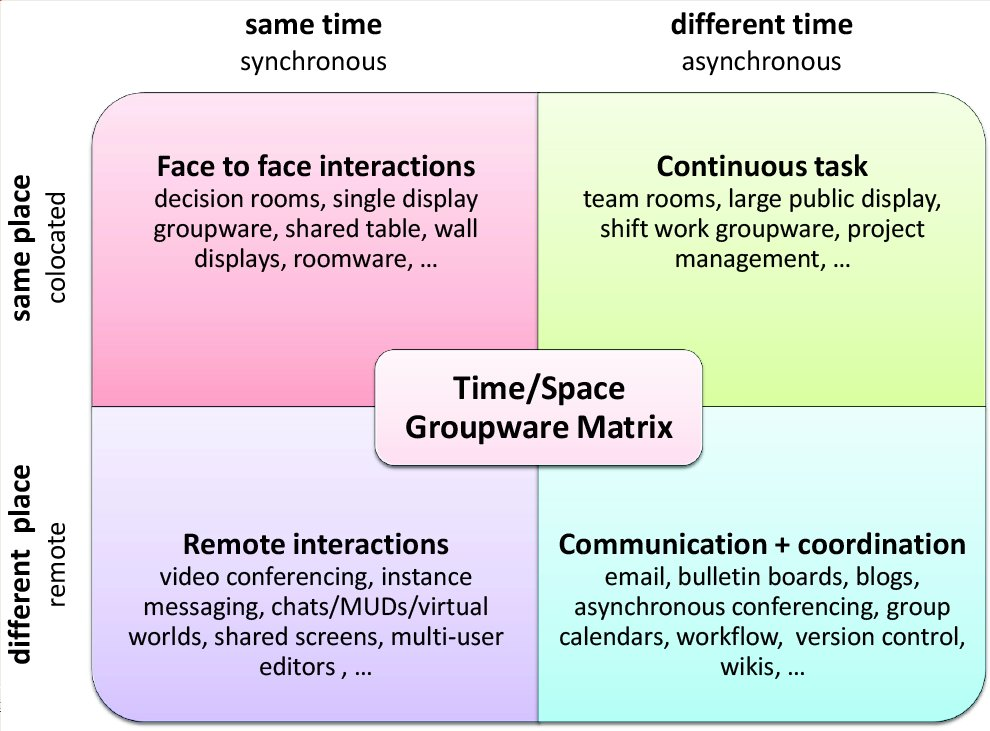
\includegraphics[width=7.5cm]{Cscwmatrix.jpg}
\caption{Johansen's Space Time matrix \protect\cite{cscw-matrix-figure}.}
\label{fig:cscw-matrix}
\end{figure}

\subsubsection{Next Sentence}
The most similar of these researched games is ``Next Sentence'', a mobile application available for Android and iOS.   


%which displays these issues in its attempt to create a game similar to ``Word Spud'' in the remote asynchronous domain \cite{next-sentence, word-spud}. 

Next Sentence, created by Ripple Digital Publishing, is a cognitively distributed game where participants take turns adding a full sentence to a story they are only given a few prior words to\cite{next-sentence-how}. A player's turn starts with seeing the title, and the last couple of words added, followed by adding their own sentence. Being limited to only seeing the last couple of words creates a lack of consistency in the game, leading to players not knowing the full context of the story when it's their turn to play. In addition, the player is not limited by a time limit or turn order, allowing any player using the Next Sentence app to add additional sentences to any story, even if they were the last player. This interface is shown in Fig.\@~\ref{fig:next-sentence:home-page} and Fig.\@~\ref{fig:next-sentence:game-play}. Each story may have unlimited players, but the story as a whole has a limited number of turns set during the creation of the game.

% ***************DON'T FORGET ABOUT THIS PART********************
% ***************************************************************

%In terms of the MoCA framework, Next Sentence is asynchronous, remote, has few communities of practice, low nascence and is short-term. By design, however, it could have a large or small scale and both high and low turnover rates for any particular game.
%\newline
%\newline


\begin{figure}[H]
\hfill
\subfigure[Next Sentence Home Page \label{fig:next-sentence:home-page}]{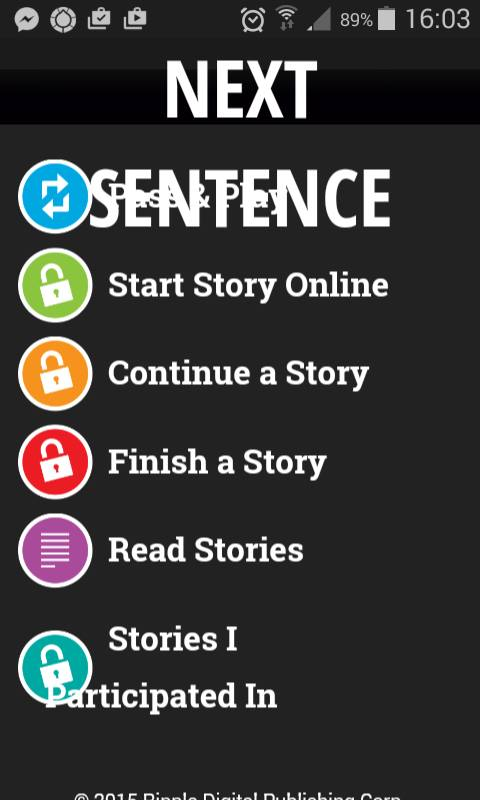
\includegraphics[height=6cm]{next_sentence.jpg}}
\hfil
\subfigure[Next Sentence Game Play Page \label{fig:next-sentence:game-play}]{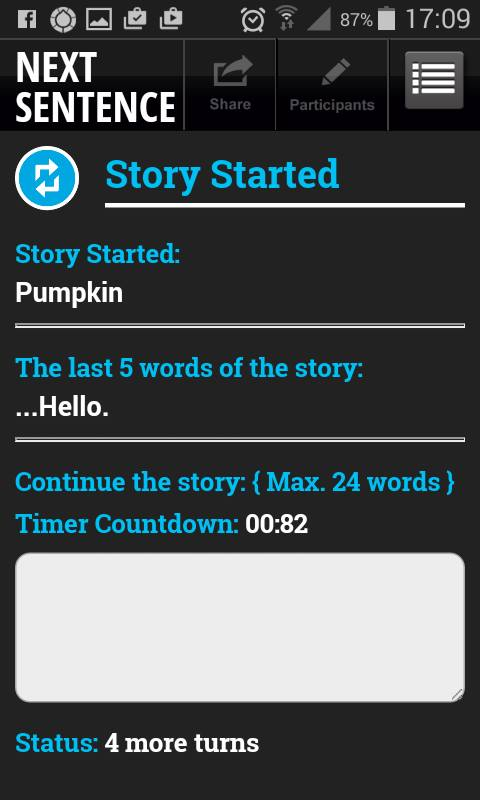
\includegraphics[height=6cm]{next_sentence_2.jpg}}
\hfill
\caption{Next Sentence Application Running on an Android Device}
\label{fig:next-sentence}
\end{figure}


\subsubsection{Words with Friends}
Another popular word game, ``Words with Friends'' available through Facebook and on mobile devices, was forced to undergo a similar change in Johansen's time-space matrix, from co-located and synchronous to remote and asynchronous \cite{cscw-matrix, words-with-friends}. Words with Friends, which is very similar to the classic board game Scrabble, is a computer supported game taking place on a virtual board for two players \cite{words-with-friends-rules, scrabble}. The players take turns using lettered tiles to place on the board in a way that words form in horizontal and vertical configurations. Doing so, creates points based on the complexity of the word and rareness of the letters used. The player with the most points at the end of the game is declared the winner \cite{words-with-friends-win}.

Words with Friends was able to overcome its transition from co-located and synchronous, to remote and asynchronous by making adaptations. For instance, using all of your word tiles at the same time is worth less in Words with Friends than with Scrabble due to the ability for the player to run anagram tools on their phone without their opponent's knowledge. \cite{wwf-vs-scrabble}. Also, since Words with Friends is not played face to face like Scrabble, they attempt to resolve that by displaying avatars of each player above the game board interface.

\subsubsection{MoCA Evaluation}
Table~\ref{tab:moca_table} shows an evaluation of StoryTime With Friends and the related games we discussed using the MoCA framework. Based on our motivation to translate our game into an asynchronous and remote environment, we decided to use the MoCA framework as it provides an analysis that covers not only physical distribution and synchronicity, but also other useful dimensions. We wanted to find were differences between our game and other similar games using the seven dimensions of the MoCA framework. This analysis helped us determine the scale and turnover rate of our game. Next Sentence had an extremely large scale and a high turnover rate. An unlimited amount of players could join the game and leave as they wish. By analyzing this feature, we have concluded that by limiting the number of players who could join the game, they would have more opportunities to input words into the story and become more engaged. This may then lower the turnover rate as players will not leave to find a game that had less players.

\begin{table}[H]
\centering
\begin{tabularx}{\linewidth}{ >{\small}l | >{\raggedright\small}X | >{\small\raggedright}X | >{\small}l }
 &
StoryTime With Friends &
Words With Friends & 
Next Sentence \\ \hline \hline
Synchronicity & Asynchronous & Asynchronous & Asynchronous \\ \hline
Physical Distribution & Distributed & Distributed &  Distributed \\ \hline
Scale & 10 {\footnotesize players} & 2 {\footnotesize players} & Unlimited \\ \hline
NCoP & Small & Small & Small \\ \hline
Nascence & Moderate & High & Low \\ \hline
Planned Permanence & Moderate & High & Low \\ \hline
Turnover & Moderate & Low & High \\ \hline
\end{tabularx}
\caption{Evaluation of Words With Friends, Next Sentence, and StoryTime With Friends using the MoCA framework}
\label{tab:moca_table}
\end{table} 
 


% ***************DON'T FORGET ABOUT THIS PART********************
% ***************************************************************

% Based on the above explanation, Words with Friends is asynchronous, remote, has few communities of practice, is low nascence, short-term, small scale, and has a low turnover rate.
%\newline

% *******INCLUDE A TABLE SUMMARIZING THE MOCA FRAMEWORKS FOR THE ABOVE MENTIONED GAMES********
% *************AND EXPLAIN WHY WE USED THE MOCA FRAMEWORK AND HOW IT HELPED*******************

\subsection{Related Literature}

\subsubsection{Impact of Collaborative Games}
The article ``Collaborative Games: An Exploratory View for Instructional Designers'', written by Jason Drysdale of the University of Colorado, examines the value of collaborative games as team building and collaboration tools within team-based work environments \cite{drysdale2011collaborative}. It was found that more people identify themselves as gamers today than in the past, with 69 percent of heads of households and 97 percent of children playing video games. It is also noted that every one of four gamers is over 50 years old, with the average gamer being 30. Since the demographic of gamers has grown, video games have become more mainstream and can be a valuable medium for learning skills desired by most organizations if designed with collaboration in mind. Games provide many opportunities to develop and enhance teamwork and leadership skills; because of this many organizations use games as a way to provide content in a more fun and exploratory way to employees. There are three subgroups to collaboration within a collaborative game: cooperating, coordination, and co-creating. Our game, StoryTime with Friends, has all three of these subgroups, making it a good candidate for enhancing team building and collaboration skills. Cooperation comes into play because players must take turns in adding words to the story based on a theme provided by a generated title. Coordination comes into play because in order for the story to make sense players must coordinate their individual input to flow with the rest of the story. Lastly, co-creating is the main focus of our game since the goal is to create a story as a group.

\subsubsection{Distance Work}
In the workplace, distance plays a large factor in what makes a distributed team successful. Distributed teams are often made up of people from different backgrounds to produce a variety of ideas. \cite{distance} For the sake of our game, StoryTime with Friends, distance is one of the main factors of changing the time-space matrix of Story Time, the Sociables rule.

The common stressors that distributed teams face are:
\begin{itemize}[leftmargin=.5in, noitemsep]
\item Blind and invisible
\item Time-zone differences
\item Crossing institutional or cultural boundaries
\end{itemize}

The first stressor, blind and invisible, is when people on a team are invisible to those that are not at their location, and therefore must communicate and coordinate explicitly. StoryTime with Friends is played remotely with players contributing words to the story using their own device. They are able to see whose turn it is and how many people must take a turn before they are able to take theirs, but are ``blind'' about the activity of the other players until the newly added words appear when a player has finished their turn.

Due to the nature of the game being remote and asynchronous, playing with multiple people across different time zones may cause one to wait a long time until it is their turn again. In the MVP of our game we will provide a time out feature, where a player's turn will be skipped if they are inactive for too long.

When crossing institutional or cultural boundaries in the workplace, conversational or decision-making practices and expectations may differ. This may also occur while playing StoryTime with Friends with people from different cultures. The story that has been written so far may not make much sense to someone, or certain words may have different meanings. 

\subsubsection{Distributed Cognition}
Distributed cognition is the psychological theory that an individual is not the only one containing knowledge, but that the individual's social and physical environment does as well. There are three ways that cognition can be distributed: 
	
\begin{enumerate}[leftmargin=.5in,noitemsep]
\item Cognitive processes may be distributed across the members of a social group.
\item Cognitive processes may be distributed in the sense that the operation of the cognitive system involves coordination between internal and external (material or environmental) structures.
\item Cognitive processes may be distributed through time in such a way that the products of earlier events can transform the nature of related events. 
\end{enumerate}

Our application touches on all the previously mentioned ways of distributing cognition. Since StoryTime with Friends users will be able to each add their own words to a shared story, cognition will be distributed across the members of the social group participating in the game. Also, because we are adapting the original game idea to be computer supported, the operation of the cognitive system will involve coordination between internal and external structures. The internal structure being the participating players individual contributions to the story, and the external structure being the computer supported environment supplied by the application that displays the end product of all those contributions. Lastly, the fact that users are able to see the story unfold as they wait for their next turn can change the words they choose to input when it is their turn once again. This ties into the third way that cognition may be distributed as listed above.

\newpage

\section{Design Rationale}
As stated in the introduction, our goal is to implement a computer supported version of the orally played game, Story Time. In order to achieve this goal, we looked at some adaptions that needed to be made to the oral version so that it would translate well to a computer supported environment. We came up with multiple features that could be implemented within the game to support these adaptations. Here is a list summarising those features and the rationale behind them:
%%
\begin{enumerate}[leftmargin=.15in,noitemsep]
\item Players can input four words into the story each turn.\\

The original version of Story Time requires each player to add only one word to the story at a time. However, to avoid players getting stuck with inputting little words like \textit{and}, \textit{the}, \textit{a}, etc. , we wanted to allow players to enter at least four words each turn in order to make it more fun for each individual. We picked this limit so it would make it hard for players to enter a whole sentence, that way we could keep the spontaneity of the original version and allow other players the opportunity to steer the story in different directions mid sentence. \\

\item Players can choose from a set of tiles each turn. Each tile has a few words on them.\\

We came up with the idea for this feature because we were initially trying to think of a way to include a points system to make Story Time fit the formal definition of a game, which would mean there would have to be a win or lose outcome. In the end, even though we decided against implementing a points system, we wanted to test the idea of using word tiles versus inputting four words as the main game play feature. Since us, as the developers, thought it was an interesting idea, we explain this further in our Design Phase One section below. \\

\item Randomly generated story title.\\

The verbal version of Story Time does not require the story being created to have a title. However, in our game, players could be participating in multiple stories, therefore we needed a way to be able to list on-going, and completed stories in a way that players can differentiate stories easily. Instead of allowing people to create their own title, we provide them with a randomly generated one. We also decided to do this to make the game more interesting by adding the element of writing a story following the theme presented by the random title.\\

\item Set the number of turns per person.\\

We decided to allow users to set the amount of turns each player gets per game. That way they can decide how long they want a game to last. We also did this to decrease the possibility of stories being left incomplete. \\

\item Time limit to complete a turn.\\

The verbal version of Story Time is synchronous and co-located, therefore players have more pressure on them to add to a story in a timely manner; and because they are face to face they complete a story from start to finish in one sitting. Since the computer supported version of Story Time we are implementing will allow for asynchronous play, we needed to implement a way that would limit the amount of time a user has to wait for their next turn. This way players will not get bored and give up on a story. To combat this, we allow the creator of a story to set a time limit for turn completion. If a player does not successfully contribute to a story in the set time limit during their turn, they will be skipped, and the story moves on to the next player.\\

\item Invite friends to write a story.\\

Since our version of the game is played online, and players are most likely distributed among different locations, we needed a way that they can connect to other players in order to start creating a story with each other. Therefore, we have provided an invite friends feature to use when starting a game.\\ 

\item Chat.\\

Unlike the oral version of Story Time, users will most likely not be in the same place while collaborating on a story. So, we thought about adding a chat feature to help facilitate the loss of communication.

\end{enumerate}

%%
%\section{Methodology}
%%
%We have conducted user studies that includes an interview and a demographic survey in order to collect data to be used for qualitative analysis. This section will thoroughly describe our StoryTime with Friends prototype, the user evaluation process, data analysis and conceptual design.
%%
%%
\section{Design Phase One} % **Might want to rename it?

\subsection{Prototypes}
Using the prototyping tool provided by www.proto.io, we created two prototypes of StoryTime with Friends. These prototypes were created based on ideas in early design discussions, where we wanted to ensure the game was fun and engaging for our users. The idea of having word tiles was brought up, therefore, we believed that giving users two prototype versions (non-tiled and tiled) would help us determine which one they preferred. 

For the first prototype (Fig.~\ref{fig:prototype:non-tiled}), players are given the ability to contribute four or less words to the story during their turn. In the second prototype (Fig.~\ref{fig:prototype:tiled}), players are restricted to choosing one out of six tiles containing four or less words. This helped us decide whether the player enjoyed having the freedom to add their own words or would rather select from a pre-determined set of words.   

\begin{figure}[H]
\hfill
\subfigure[Non-tiled Version \label{fig:prototype:non-tiled}]{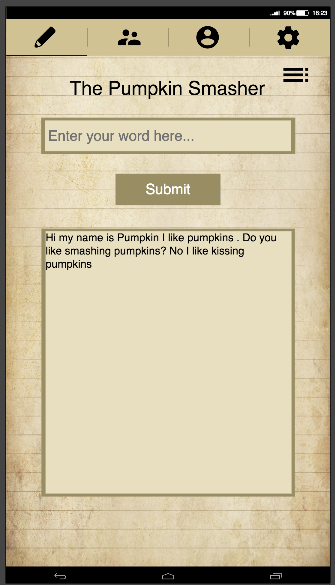
\includegraphics[height=6cm]{image01.png}}
\hfill
\subfigure[Tiled Version \label{fig:prototype:tiled}]{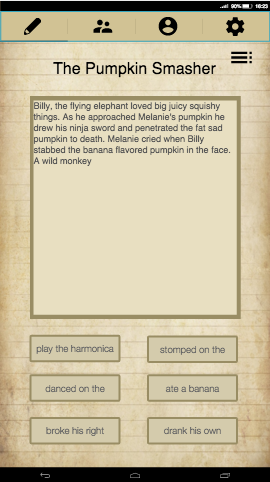
\includegraphics[height=6cm]{image02.png}}
\hfill
\caption{Prototype Used During User Test for StoryTime With Friends}
\label{fig:prototype}
\end{figure}

Due to unforeseen bugs when exporting our prototype onto a mobile device, we were forced to conduct the gameplay on a laptop. The participants were told to imagine that they were using a mobile device and had to pass around the laptop after each turn. 


\subsection{User testing}
The three main objectives of the user testing session were:

\begin{enumerate}[leftmargin=.5in,noitemsep]
\item To observe the participants while playing the game.
\item To determine the enjoyability of our game.
\item To discover features and requirements for the game (number of players per story, time limits, number of input words per turn, etc).
\end{enumerate}

All the participants involved in the user testing were UVic undergraduate students between the ages of 18 to 24. We decided to select them as our target audience because university students typically have good background knowledge of various computer technology and games. We believe having a specific target audience for interviews generates more accurate and consistent results. Due to time constraints, limited accessibility, and indications in our ethics application, we were unable to involve a wider demographic of participants in this study. 

We conducted two user testing sessions, the first session consisted of four players, and the second session consisted of five players; both were conducted in the exact same manner. An explanation of our game was provided to the participants, followed by them answering simple demographic questions (see next section). Next, we watched the participants as they used our prototypes. The first prototype they were given to use was the tiled version, followed by the non-tiled version. When they had finished playing, we interviewed the participants regarding their experience during the gameplay. The interviews were audio recorded and transcribed for further analysis.

%\subsection{Data Analysis}
For privacy and ethical reasons, we replaced the names of our participants with code names after linking the data of each section (demographics, interview, and environmental study) together. The transcribed audio recordings were placed in a shared document, and the summarized answers to the questions were placed in a table.

\subsection{Demographic Questions}
Before participants played with the prototypes, we asked them to answer a few demographic questions. The purpose of this was to give us a better understanding of our participants, and analyze how their demographics may influence their gameplay or answers to the interview questions. 

The following demographic questions were asked:
\begin{enumerate}[leftmargin=.5in, noitemsep]
    \item Have you ever played Story Time game? (never, a few times, many times)
    \item Have you ever played other types of word games? (never, a few times, many times)
    \item Have you ever played collaborative computer games? (never, a few times, many times)
    \item How frequent do you play computer games? (never, a few times a year, every month, every week, every day).

\end{enumerate}

\subsection{Demographic Question Responses}
Although we had a low number of participants, the demographic questions were able to help us determine whether they were familiar with the Story Time game or had played any other types of word games. As seen in Fig.\@~\ref{fig:demographics}, a majority of our participants (six out of nine) stated that they had played other types of word games before and many had played collaborative games as well. This reinforces the selection of our target audience and the assumption that university students have good background knowledge of computer technology and games.  

\begin{figure}[H]
\centering
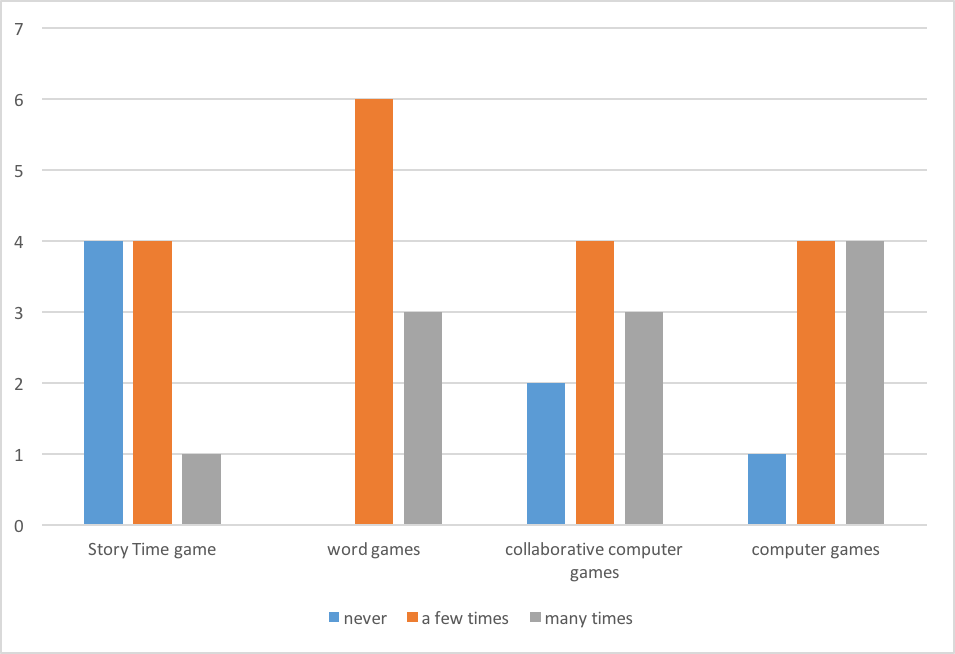
\includegraphics[width=0.4\textwidth]{demographics.png}
\caption{Interview Participants Previous Experience With Games}
\label{fig:demographics}
\end{figure}


\subsection{Interview Questions}
Following user testing, each participant was interviewed individually about their experience. The interview questions were designed to target the three objectives that was previously mentioned, and assist us in determining which features should be included.

Below is the list of the interview questions we asked the participants:
\begin{enumerate}[leftmargin=.5in, noitemsep]
    \item Did you prefer playing version one (input any words), or version two (choose from the given tiles of words) of the game? 

    \item Did you like being given a random title for the story, or would you have preferred inputting your own title?

    \item This relates to the non-tiled version of the game. How many words do you think should be the maximum per turn?

    \item Would you download and play our game with your friends (if it was free)? Why or why not?

    \item We were thinking about limiting the amount of time the game takes, or the amount of time a player is allowed per turn by introducing a time limit. Do you think that the game should be time limited in some way? We would like to know your opinion for both the tiled version, and the non-tiled version of StoryTime.
        \begin{itemize}[noitemsep]
            \item If so, how?
        \end{itemize}

    \item How many participants should partake in a game? (please answer in a range)
    
    \item Do you think a chat feature would be useful for this game? Why or why not?
    
    \item If you were allowed to play both public games and private games with friends, which one would you played more?
    
    \item Were there any features that were missing which you would have liked to see from the gameplay?
\end{enumerate}


\subsection{Interview Question Responses}
After analyzing the responses to the interview questions, we categorized the answers into nominal data. Appendix~\ref{apx:interview-responses} presents the summarized results in a table. 

From the responses gathered from the interviews, we found that the participants preferred to have a time limit. 

\thinspace \thinspace
``\textit{... I think it [time limit] would add an element of pressure to the game, and you would not sort of be sitting there waiting for someone to come up with the perfect sentence... especially for the first [tiled] version if you're having to write your own stuff. Like waiting for someone to concoct their own thing, it would definitely get passed around really quick, and that would be kinda... it would imitate more the live version. Like if you're taking off the Sociables version where everyone is going around in a circle it would better emulate that. If you were doing the second version uhmm... you could have an even shorter time limit. That it's like, you just have to take your first instant reaction, and that could be cool too. You could make a really fast game like that.}'' %\textit{Apollo}\thinspace \thinspace  

When asked the same question, \textit{Dionysus} mentioned the difference of having a time limit for remote games over in-person games. He says:

\thinspace \thinspace ``\textit{If you're playing alone on the internet (with random people) then yes. You would want it to be a faster game. But if you're with your friends I would say you don't really need a time limit.}'' \thinspace \thinspace

In regards to being given a random title or inputting their own title, the majority of participants (six out of nine) had expressed preference in being given a random title. For instance \textit{Demeter} said:

``\textit{I like when the title is there, it kinda just helps get the game going... having a theme chosen for you}''\thinspace \thinspace 

\textit{Athena} also gave an interesting suggestion that we had not thought of before: 

``\textit{In a game scenario, I think to be able to re-generate the random title, maybe a maximum of 3 times, will be cool. The third time you'll just have to go with that one.}'' \thinspace \thinspace

\subsection{Observations}
We watched the participants while they were playing with both versions of the game to see their behaviour and reactions. For instance, they were seen laughing while reading the story during their turn for both the tiled and non-tiled version of StoryTime with Friends. This satisfies one of our main objectives of ensuring the game is funny and entertaining. 

We also found that for the non-tiled version, some participants took up to two minutes to read the story and input their words, while others did not take as long (approximately 30 seconds). Due to the various reading abilities of players, as well as the length of the story, it is difficult for us to determine a viable time constraint for how long a player has to play their turn. More importantly, this user testing was accomplished in a synchronous and co-located time-space matrix, which made games much faster. But a time limit was required to ensure that games are not ``stuck'' at one player's turn, so in this stage we decided to put a 24-hour time limit for each turn.
%Players will be able to take as much time as they need to read the story and input their words, but there will be a time constraint for how long it takes for them to return to the game, which begins as soon as they receive a notification letting them know it's their turn. This will ensure that the game is not ``stuck'' at one player's turn and will keep the game moving along.
\newline

\section{Design Phase Two}

\subsection{Design Decisions}
When designing the MVP, we had to determine what we would implement and what changes we would make to the prototypes developed in the first phase. We used the feedback from the user testing session and made the following decisions: 
\begin{enumerate}[leftmargin=.15in,noitemsep]

\item Players can input four words into the story each time.\newline

After the user testing with the two different prototypes in the first design phase, we were able to decide to go with the non-tiled version of our game, where players input four words into the story each turn. This is due to the fact that out of the interviews we conducted after the prototype testing, eight out of the nine participants preferred the non-tiled prototype. We also asked participants to provide us with a range dictating how many words they thought would be appropriate to input each turn. Based on the feedback we decided to stick with our original idea of four words per turn.\newline  

\item Keep the randomly generated story title.\newline

Out of the nine participants from the user testing in phase one, six of them liked being given a randomly generated title. Therefore, we decided to stick with this feature.\newline

\item Add story title regeneration.\newline

In our user testing sessions, during our first design phase, we had a suggestion from a couple of participants to allow for the regeneration of the story title if the first one provided is not to the players liking. On top of this, it was also suggested that we limit the amount of times the title can be generated. We thought this was a good idea in order to prevent users from spending to much time looking for the perfect title. So we decided to only allow the user to regenerate the title up to three times.\newline

\item Allow users to set a desired time limit per turn.\newline 

Seven out of the nine participants from our user testing in design phase one said yes to having a time limit to complete each turn. We deferred the decision about the actual amount of time to the users of the application because each game contains a unique set of participants with varying circumstances. Therefore, we wanted to give them the opportunity to decide how long a game will last.\newline

\item Allow users to specify number of turns in a game.\newline 

This feature ensures that a game can be customizable with concerns to the circumstances of participating players, while also inducing an end to the story. In addition, it provides an equal amount of turns per player.\newline 

\item Add colour codes for user input and turn highlighting.\newline

From self-testing we found that not being aware of who input what words, as well as not mentioning who the next player is, might cause the participants to feel disconnected from the other players. Therefore, we considered colour codes for user input and turn highlighting to be a viable feature and had it implemented.\newline

\item Add turn notifications.\newline

Since StoryTime With Friends is an asynchronous game, the story would sometimes stall because a player is unaware it is their turn. Although we previously thought an implementation of a notification system would be done in the future work of our project, we found that a basic email notification system was necessary. \newline

\item No Chat feature.\newline

Unlike the oral version of Story Time, users will most likely not be in the same place while collaborating on a story. So, we thought about adding a chat feature to help facilitate the loss of communication. However, during user testing in the first design phase, we found that most users thought that a chat feature was not a necessity for the game. 

\end{enumerate}

\subsection{Conceptual Design}
After deciding on the general features and design of our MVP, we needed to create a conceptual design, available in Appendix~\ref{apx:conceptual}. We did this in order to assist in creating the user interface for the Minimum Viable Product, allowing us to easily notice any missing components in our game prior to the implementation. The conceptual design was planned out using an online, collaborative, diagramming tool called LucidChart. This tool makes it easy to create and share flowcharts, mockups, UML (Unified Modeling Language) diagrams, mind maps and more.

\subsection{Implementation}
Each of us were involved with the implementation process. Three of us were focused more on back-end, and the other two on front-end development. To enable parallel team development, we created a three-tiered framework using the Model-View-Controller design pattern to separate application logic from the presentation layer and started coding the application on top of that. Fig.\@~\ref{fig:mvp} shows the interface of a sample finished story.

\begin{figure}[H]
\centering
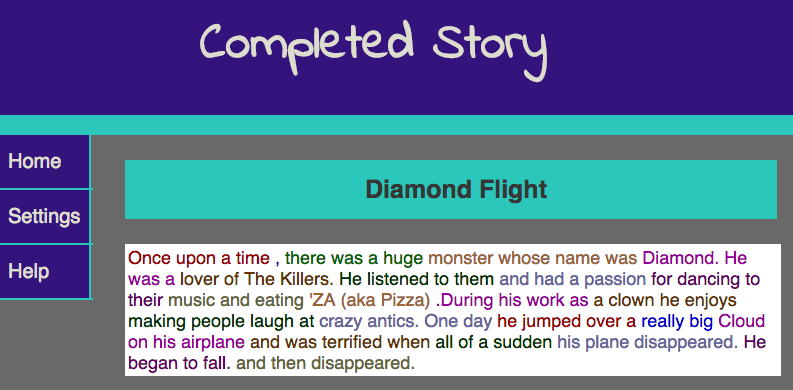
\includegraphics[width=0.4\textwidth]{mvp.png}
\caption{A finished story in the MVP interface}
\label{fig:mvp}
\end{figure}

\subsubsection{Technical specifications}
Here is the detailed list of tools and technical specifications we used for implementation:

\begin{itemize}[leftmargin=.3in,nosep]
\item cPanel as web hosting control panel
\item phpMyAdmin, HeidiSQL and Sequel Pro as database management clients
\item GitHub allowing for version control and collaboration
\item PHPStorm, WebStorm and Cloud9.io as development environments
\item PHP as server-side programming language
\item Apache as the web server
\item MySQL as the relational database management system
\item HTML and CSS3 for front-end presentation
\item JavaScript programming language and JQuery library for front-end programming
\end{itemize}

\subsection{Self-testing}
Before going into the second round of user testing, we decided to test it ourselves. We tested it both synchronously and asynchronously to find out potential shortfalls. Based on our own experience, we revised two minor design decisions followed by making some implementation enhancements. We decided to allow the users to input the amount of time for each turn, and also showed them details about who put certain words to prevent players from feeling disconnected from each other.

\subsection{Evaluation Design}
To design the final round of evaluation, we defined two main objectives while taking into consideration our motivation behind the project. First, determine whether participants liked our design decisions and believed that the adaptations were appropriate for the new environment to maintain the same enjoyable experience as the face-to-face version. Second, allow them to identify what they did not like from the remote experience, to assist us in creating the game to be well adapted to the remote and asynchronous space. We considered several aspects to decide the best evaluation approach and questions to be asked: our own experience from self-testing the game, responses from the interviews in the prototype user testing session, observations of participants playing with the prototypes, and various constraints such as lack of time. 

Although it was hard to accomplish, we asked both old and new participants to test the game while they were distributed throughout different locations. As a result, we were unable to observe almost half of participants while they were playing. We decided to choose a questionnaire over an interview, since we did not need any follow-up questions. From our experience in the interviews, we decided to not include any general open-ended questions where participants would have trouble answering or did not have enough background knowledge to answer appropriately. For example, asking participants which features they think should be added to the game was difficult for many participants to answer. Instead, we asked them about their experience with the game and used their answers to determine what they would have wanted and what is missing from the game. We also included some feature-related questions similar to those asked in the first round to see whether their opinion had changed after experiencing the remote game.

\subsection{User Testing}
In the short amount of time we had to complete our user testing for the MVP we were able to get 10 participants. There were a total of three games played by different sets of participants at different times. One game consisted of five participants, another consisted of three, and the final game was played with two. We asked them to fill out a questionnaire, which we made using Google forms. The complete questionnaire is available at \url{http://yon.ir/StoryTime}. Here is a quick list of the questions we asked: 

\begin{enumerate}[leftmargin=.5in, noitemsep]
    \item Did you find the time limit to be needed?
        \begin{itemize}[noitemsep]
            \item If yes, would you make any changes to the amount of time allowed per turn?
        \end{itemize}    
        
    \item Did you like the random title generation?
        \begin{itemize}[noitemsep]
            \item If yes, did you like the random title generation constraint on limiting titles?
        \end{itemize}
        
    \item Did you like having a turn constraint?
    
    \item Did playing story time in a different space than other participants, rather than in the same space together, change how you provided input to the story?
    
    \item Recall your experience playing StoryTime With Friends. What emotions and thoughts did you have while playing the game?
    
    \item Did you ever feel disconnected from the other players while playing? Why did you feel this way?
    
    \item Would you play our game again?
        \begin{itemize}[noitemsep]
            \item Why or why not?
        \end{itemize}
    
\end{enumerate}

\subsection{Questionnaire Response Analysis}
Appendix~\ref{apx:questionaire} presents the complete list of results to the questionnaire in a table. After reviewing those responses, we found them pretty biased which did not make them valuable for quantitative analysis. However, we found some of the responses useful and worth mentioning. For instance, in response to the question ``How likely would you be to play StoryTime With Friends? Why?'' \textit{Themis} said:

``\textit{Somewhat, likely. It is fun, I can see it becoming a popular mobile game, but one that would/could die off after a month or so with close friends.}''

This response raises the question that if StoryTime With Friends does die off quickly, would it be specifically because of our online version of the game or the real world game itself? It is important to consider that games are often short-lived, as gamers move quickly from one game to the next. To enforce the longevity of StoryTime With Friends, more features will need to be tested and evaluated to ensure a non-repetitive and exciting environment is maintained. 

Another useful response we received was to the question: ``Recall your experience playing StoryTime With Friends. What emotions and thoughts did you have while playing the game?'' The same respondent, \textit{Themis} replied with:

``\textit{It was fun to play, especially while playing with a like-minded person. I enjoyed the customizable options for number of turns and so on, would be nice to customize the response time needed for individual games.}''

What we found interesting about this response was that the participant enjoyed playing with like-minded players. This may motivate some future work to include a grouping system for the different personalities of individuals.  

\section{DISCUSSION}
\subsection{Unexpected Findings}
Contrary to our initial assumption that participants would enjoy the tiled prototype of StoryTime with Friends more than the non-tiled prototype, we found that eight out of nine participants favoured the non-tiled version. Based on the interview responses, the participants preferred having the freedom of inputting any words they liked, rather than being restricted to the six sets of given words.

We also believed that having a chat feature might be necessary to enable players to share their experience and feelings while playing the game. We did not end up implementing a chat feature based on participants feedback after prototype testing, and from questionnaire responses it also doesn't seem to be necessary. However, we still believe that such a feature might be vital in the future based on our own experience of self-testing. The biased nature of the MVP evaluation responses as well as the time-space matrix difference of the prototype evaluation may be accountable for this inconsistency.

\subsection{Synchronous Space Potential} 
After the implementation of our MVP, we set up a running StoryTime with Friends game for the class to play during out final report presentation. Although originally included as a way to make the presentation a more engaging experience for the audience, it allowed the MVP to show promise as a synchronous experience. Seven participants from the audience worked together to complete a story live in front of the class with turn limits of 60 seconds.

While the synchronous and co-located nature of the demo is not part of our motivation, nor is planned to be part of the goal of StoryTime with Friends, it does provide valuable insight. For instance, we noticed that there were multiple turns missed. In addition, from the discussions among players, we noticed that they found it interesting to know who put up what words, so that they could comment on each others additions to the story. There were multiple instances of laughter or intense concentration caused by the game, and players seemed enthusiastic while playing it.

It should be noted that the demo we gave in front of the class was done in a non-formal manner. Although no formal verification was done of the results displayed in the class by the demonstration, it does allow us to know that StoryTime with Friends could be brought back to the original synchronous and co-located time space matrix in it's current form, and still be successful. This strongly suggests that the ``core'' of the game has been maintained through all the changes we made to Story Time to translate it to the asynchronous remote point on the time-space matrix.


\subsection{Lessons We Learned}
In this section, we will highlight the lessons we learned during the process of researching and implementing StoryTime with Friends. The following is a list of lessons we believe can be applied to future work:
%%
\begin{enumerate}
\item Stick with your motivation throughout all decisions.\\

One of the first discussions we had as a team - after deciding that we wanted to bring Story Time to the online game world - was to brainstorm features for the game that would be fun for the players. These included features such as providing tiles of words to choose from, a point based system to determine winners of a game, and a voting system to ``kick'' players out of a game. However, we found that these features would provide a bias to our result on whether the game has been successfully translated to the online world, as these are added features that were not present in the original real world game. Therefore, we kept added features to a minimum and ensured all features of the real world game had been implemented. The features we did add were the random title generator and the ability to input four words, instead of one, to the story. The reason behind these two additions were discussed under the Design Rationale section.

\item Ensure proper articulation work is done before getting user feedback.\\

Due to time constraints and the participants for our MVP evaluation being distributed, they were not able to play the real world co-located version of Story Time beforehand. To properly evaluate the success of our translation of Story Time to the online world, we wanted to acquire concrete answers from participants to the question of:\\

\textit{``Did playing story time in a different space than other participants, rather than in the same space together, change how you provided input to the story?''}\\

An answer of ``no'' would indicate that our translation of the game has been successful. Our implementation of the color codes to determine which player input which words in the MVP increases awareness and helps participants to not feel differently when providing words to the story whether they were playing the real world version or playing online. However, we did not receive proper feedback to this question as not all participants have played the real world version of Story Time. We've learned that it is important to focus more on the articulation work that goes into conducting a user evaluation.


\item With regards to qualitative data, interviews provide more informative and less-biased responses.\\

For our prototype evaluation in the first design phase, we conducted interviews for data collection to get a better understanding of participants' feelings throughout their game experience. For the MVP evaluation, we thought that questionnaires might provide better responses by allowing participants to have more time to think about their answers. However, after getting the questionnaire responses back for the second design phase, we found them very biased, short, and uninformative. We determined that a questionnaire is usually a good option when you want to achieve quantitative data. When designing a questionnaire, we suggest using multiple choice or yes/no questions. Although there is not enough time to do another evaluation, it gave us an important lesson to be considered in our future work as well as provide some useful feedback.

\item Reduce external dependencies to increase accessibility.\\

This one ended up being a late lesson for us in that we were unable to incorporate its lessons in time for this report. During our in-class final presentation, we had the audience participate in a live game by signing up for our service, and telling us the name they signed up with. This became an issue since the only way to register with StoryTime with Friends is to use your Facebook account, which caused some audience members who did not want to share their Facebook, or did not have a Facebook account to become reluctant and not participate. It would have increased the number of participants we had if we offered an alternative method of signing up for StoryTime with Friends.

\end{enumerate}

\section{LIMITATIONS}
Although we changed the time-space matrix of Story Time and made it possible for people to play the game remotely and synchronously, there were some limitations that impacted both design decisions and evaluations. 

Due to time constraints, our user test results were limited to the small amount of participants who were available to test our MVP and play our game and respond to follow-up questions. With a small amount of participants, the data collected was not as diverse and did not fully represent our target audience. The user testing should have been conducted earlier to involve a larger group of participants and had more participants who had originally tested our prototypes. 

Contrary to what we expected from using a questionnaire instead of an interview, we received very biased feedback in the user testing of our MVP. This deprived us from having an evaluation that was honest and insightful. Initially, we assumed participants would be more honest when responding to the questionnaires, as their identities would remain anonymous. Unfortunately, this seemed to not be the case, as many of the responses seemed to be rushed and dismissive. Moreover, a large majority of the participants playing the MVP in a remote and asynchronous space did not have the experience of playing the oral version and/or synchronous computer supported one. By not having this background, the participants were unable to provide us with insightful responses which could help us evaluate our adaptations.

\section{FUTURE WORK}
For the purposes of implementing a Story Time game in the asynchronous remote space, there is still a lot of work that is required to be completed before a finished product is ready. We believe that the following items are the core issues to be addressed: 
\begin{enumerate}
\item Additional user testing. \\

The majority of our design decisions were based around feedback from user testing, which allowed the product to grow organically, and in the direction required to improve user experience. The cycle of getting user feedback, and then implementing that feedback should be repeated multiple times in the future in order to reach a finished product.

\item The application should provide additional feedback to the user. \\

In the current product, it is not clear in what state the application is in to the user. For instance, the create story button will take you to the new story page even if you are not logged in, but will fail to create a story due to not being logged in. The main page will display an empty list of stories instead of prompting to log the user in to see their stories. These feedback points for the user's should be corrected before continuing.

\item Additional support for the game's asynchronous nature. \\

StoryTime with Friends currently requires additional support to help keep users engaged with it's asynchronous nature. We recommend adding a better notification system that are sent during the beginning of a user's turn in order to ensure that users continue to play their turns in a story in a timely manner.

\item Communication support between players. \\

During self-testing and second round testing, we found that awareness between players was lacking, and believe this was caused by a lack of communication. Since communication is a key component in games and collaboration, better communication channels might need to be implemented and tested in the future. Commenting, liking, sharing, and chatting are some examples of communication channels that may be considered.

\end{enumerate}


\section{CONCLUSION}
For the purposes of this report, we attempted to translate the mini-game ``Story Time'', from the game Sociables, from the synchronous co-located domain into the asynchronous remote domain. After researching similar games, we determined that there are no current applications that have successfully shifted the domain of Story Time, and decided to implement it ourselves with two main goals:
\begin{itemize}[leftmargin=.5in,noitemsep]
\item Ensure that StoryTime With Friends is a game that players will enjoy and find amusing. %From the feedback we have received, we believe the majority of people who have played our game found it enjoyable and would play it again, satisfying this goal.
\item Ensure that the game is fully adapted to its new asynchronous remote position on the CSCW-Matrix.
\end{itemize}

After doing two rounds of prototyping/implementation and user testing, we have completed a MVP that encompasses the core result of the CSCW matrix transition. However, based on the results and analysis of our user evaluation on our MVP, it is difficult to determine how successful our translation of Story Time to the online world was. Our approach to the MVP user evaluation resulted in answers that may have been biased or not applicable to the participant.

To overcome these limitations, we have given suggestions to consider in this project in future work. This will encompass solutions that result from some of the lessons we learned during our endeavour to provide a version of Story Time translated to the remote and asynchronous world.








%\section{Next Steps}

%Since StoryTime with Friends is a project that is focused more on implementation rather than research, our team will be creating a Minimal Viable Product (MVP) in order to conduct further user testing. The MVP will take into consideration the information we gathered and analyzed from our first user testing on the prototypes discussed above. Each member in our team will perform a cognitive walkthrough of the MVP prior to the second user testing.

%The MVP will be implemented as a web application, which when finalized, we intend to release as a Facebook game application. Due to the overwhelming majority of participants in our first user testing preferring the non-tiled prototype, our MVP will be implemented in this way. 

%The purpose of the MVP is to decide on the features we have discussed for StoryTime with Friends and to determine whether they will be implemented into the final product. The MVP will be designed in a way that allow players to be distributed on their own computers while playing the game. This will introduce a more realistic approach in the user testing, in comparison to the first prototype, which forced the players to pass around a single computer. It is important to note, however, that the implementation of our final product is not in the scope of this project. We will instead discuss what we found from our user testing of the MVP and provide thorough documentation on what we believe the final product will consist of and why.

%Our team has built the necessary platform in order to start the implementation process. The following are the tools we are using that allow us to collaborate on coding this application:

%\begin{itemize}[leftmargin=.5in,nosep]
%\item cPanel as web hosting control panel
%\item phpMyAdmin, HeidiSQL and Sequel Pro as database management clients
%\item GitHub allowing for version control and collaboration
%\item PhpStorm by Jetbrains as our integrated development environment
%\item PHP as server-side programming language
%\item Apache as the web server
%\item MySQL as relational database management server
%\item HTML and CSS3 for front-end presentation
%\item JavaScript programming language and jQuery library for front-end programming
%\end{itemize}


\section{ACKNOWLEDGEMENTS}

We are extremely grateful to all the participants who accompanied us during our prototype and MVP evaluations. We would also like to give special thanks to our instructor, Prof. Margaret Storey, and teaching assistant, Eirini Kalliamvakou, who have provided invaluable assistance during the course of this project.

% REFERENCES FORMAT
% References must be the same font size as other body text.
\bibliographystyle{SIGCHI-Reference-Format}
\bibliography{bib}

\onecolumn
\createappendix{Milestones}\label{apx:completed}

\begin{table}[h!]
\centering
\begin{tabular}{>{\raggedright}p{4cm}|>{\raggedright}p{6cm}|c}

\textbf{Project Milestone} &
\textbf{Description} &
\textbf{Date Completed} \\ \hline \hline

Written proposal &
Completed written proposal that describes what our project is about and the work that we will be doing this term. &
October 16, 2015 \\ \hline

Ethics application &
Ethics application and consent forms created in order to conduct interviews and prototype evaluation. &
October 19, 2015 \\ \hline

Finish prototype &
Finished creating two prototype versions of our game that will be tested by users. &
October 23, 2015 \\ \hline

Run prototype evaluation sessions &
Conducted two prototype evaluation sessions that involved participants playing with the prototypes. Interviewed participants to receive feedback and &
\makecell{October 26, 2015 \\ October 29, 2015} \\ \hline 

Analyzing data from prototype evaluation &
Transcribed the recorded interviews to analyze the data. Determined from the data which prototype version of the game and features the participants liked. &
October 27, 2015 \\ \hline

Finalize project requirements &
Discussed as a group what our project’s final requirements are and how we will be moving forward. &
October 30, 2015 \\ \hline

Conceptual design &
Conceptual design completed in order to assist the creation of our MVP. &
November 3, 2015 \\ \hline

% ** TAKEN FROM MILESTONES MET TABLE **
Interim project report &
Complete interim report which describes our current work and the progress of the project. &
November 13, 2015 \\ \hline

Finalize MVP implementation &
The creation of a web application of the game will be completed. &
November 18, 2015 \\ \hline

User testing (cooperative observation) of MVP followed by a questionnaire &
Conduct our second round of user testing where participants will play the game using the MVP and be given a questionnaire after. &
November 26, 2015 \\ \hline

Analyze and interpret questionnaire responses &
Using the data collected from the questionnaires, we will analyze and determine what the final product would have been like if we were doing the full implementation. &
November 27, 2015 \\ \hline

Final presentation &
Present to the class the work that we have completed throughout the term. &
December 2, 2015 \\ \hline

Final report &
Final report describing in detail the work that we have done. &
December 5, 2015 \\ \hline


\end{tabular}
\caption{Milestone items completed.}
\label{tab:milestones}
\end{table}



\createappendix{A Summary of Interview Question Responses}\label{apx:interview-responses}

\begin{tabular}{ | l | l | l | l | l | l | l | l | l | l | l | }
\hline
	  & Q1 & Q2 & Q3 & Q4 & Q5 & Q6 & Q7 & Q8 & Q9 \\ \hline
	Athena & non-tiled & Random Title & 4.5 & No & Yes & 3-5.5 & Maybe & Both & No \\ \hline
	Dionysus & non-tiled & Random Title & 3.5 & Yes & Mixed & 4-8 & Maybe & Both & Yes \\ \hline
	Hephaestus & non-tiled & Mixed Opinions & 4.5 & Yes & Yes & 2-10 & Yes & Both & No \\ \hline
	Demeter & non-tiled & Random Title & 6 & Yes & Yes & 4-8 & Maybe & Both & Yes \\ \hline
	Apollo & non-tiled & Random Title & 8 & Yes & Yes & 5-15 & No & Public Games & Yes \\ \hline
	Artemis & non-tiled & Random Title & 4 & Yes & Yes & 4-5 & No & Public Games & Yes \\ \hline
	Hades & non-tiled & Input own title & 5 & Yes & Mixed & 4-8 & Maybe & Public Games & Yes \\ \hline
	Aphrodite & tiled & Random Title & 4 & Yes & Yes & 4-6 & Maybe & Both & No \\ \hline
	Ares & non-tiled & Input own title & 5 & Yes & Yes & 3-6 & Yes & Family & No \\ \hline
\end{tabular}

\createappendix{A Summary of Questionaire Responses}\label{apx:questionaire}

Q1: Did you find the time limit to be needed? \newline
Q2: Would you make any changes to the amount of time allowed per turn? \newline
Q3: Did you like the random title generation? \newline
Q4: Did you like the random title generation constraint on limiting titles? \newline

\FloatBarrier
\begin{table}[ht]
\begin{tabularx}{\linewidth}{>{\raggedright}X | >{\raggedright}X | >{\raggedright}X | >{\raggedright}X | >{\raggedright}X }
 & Q1 & Q2 & Q3 & Q4 \tabularnewline \hline
Hyperion & Yes & no & Yes & N/A \tabularnewline \hline
Theia & Yes & No, it was great & Yes & It did not apply \tabularnewline \hline
Coeus & No &  & Yes & N/A \tabularnewline \hline
Phoebe & No &  & Yes & yes it made the game move along quickly \tabularnewline \hline
Cronus & Yes & No, I think it's fine the way it is. Especially if you want it just to be a casual game. & Yes & Yeah, I'm totally fine with it. \tabularnewline \hline
Mnemosyne & Yes & No & Yes & Yes \tabularnewline \hline
Themis & Yes & No. & Yes & Not necessarily, but it makes the game a little more challenging to actually match the story to the title. \tabularnewline \hline
Crius & Yes & No & Yes & Yes \tabularnewline \hline
Oceanus & Yes & no & Yes & yes because people would spend too much time choosing a title \tabularnewline \hline
Tethys & Yes & No & Yes & Yes, because it forces you to pick a title and not keep clicking it until you get one that you like. \tabularnewline \hline
\end{tabularx}
\end{table}

\FloatBarrier
\newpage
Q5: Did you like having a turn constraint?\newline
Q6: Did playing story time in a different space than other participants, rather than in the same space together, change how you provided input to the story?\newline
Q7: Why or why not?\newline
Q8: Recall your experience playing StoryTime With Friends. What emotions and thoughts did you have while playing the game?\newline

\begin{table}[ht]
\begin{tabularx}{\linewidth}{>{\raggedright}X | >{\raggedright}X | >{\raggedright}X | >{\raggedright}X | >{\raggedright}X }
 & Q5 & Q6 & Q7 & Q8 \tabularnewline
Hyperion & Yes & No &  & I laughed, i cried. I had the time of my freakin life.  \tabularnewline \hline
Theia  & Yes & No &  & It was funny \tabularnewline \hline
Coeus  & Yes & No & I follow the story line as it is shown & I found I had to concentrate harder \tabularnewline \hline
Phoebe  & Yes & Yes & had to read everything and context & thought it was fun to play and enjoyed the story that got created \tabularnewline \hline
Cronus  & Yes & Yes & There's no easy way to communicate while playing the game. So my answer is less likely to be influenced by conversation outside of the stories context. & I had fun! It was exciting to see how others would contribute to the story. It's especially interesting when the story takes an unexpected turn. \tabularnewline \hline
Mnemosyne  & Yes & Yes & When you're playing together in the same space, it forces you to think of words faster while when you're in a different space you have more time to be a bit more creative.  & I thought it was fun and entertaining.  \tabularnewline \hline
Themis  & Yes & No & No, because I would say what I wanted to say no matter what, doesn't matter if I can see the person or not. & It was fun to play, especially while playing with a like-minded person. I enjoyed the customizable options for number of turns and so on, would be nice to customize the response time needed for individual games. \tabularnewline \hline
Crius   & Yes & No &  & Better not say anything too inappropriate during test rounds \tabularnewline \hline
Oceanus & Yes & No &  & it's a really fun game \tabularnewline \hline
Tethys & Yes & No & No, because the time limit made it so that you had to think quickly. & I thought it was really fun, and it was funny seeing the story unfold. \tabularnewline
\end{tabularx}
\end{table}

\FloatBarrier
\newpage
Q9: Did you ever feel disconnected from the other players while playing?\newline
Q10: Why did you feel this way?\newline
Q11: How likely would you be to play StoryTime With Friends?\newline
Q12: Why do you feel this way?\newline
Q13: Do you have any additional comments you wish to make?\newline

\begin{table}[ht]
\begin{tabularx}{\linewidth}{>{\raggedright}X | >{\raggedright}X | >{\raggedright}X | >{\raggedright}X | >{\raggedright}X | >{\raggedright}X}
 & Q9 & Q10 & Q11 & Q12 & Q13 \tabularnewline
Hyperion & No, not at all.  & Because it's a very fun game.  & Very Likely & Because it's enjoyable makes you laugh.  & Nope  \tabularnewline \hline
Theia & Nope & Because we are all in the same room & Very Likely & It would be fun &  \tabularnewline \hline
Coeus & No & I felt that they were here & Maybe & time constraints & None \tabularnewline \hline
Phoebe & no & na & Maybe & would play at a party its kinda fun &  \tabularnewline \hline
Cronus & Not really & Although it would be nice to see where you are in respect to whose turn it is. & Somewhat Likely & I like the game. Just would like to see a more fully implemented product. & Nope \tabularnewline \hline
Mnemosyne & No & Not all games require you to be in constant communication so this one is fine.  & Somewhat Likely & I enjoyed playing it and it was fun.  & No \tabularnewline \hline
Themis & No. & Because like any other online game, you have to take real life into account, knowing that they may not be able to fully focus their time to play a properly. & Somewhat Likely & It is fun, I can see it becoming a popular mobile game, but one that would/could die off after a month or so with close friends.  & It was a fun game and would love to see it be developed further, because I think it could go far! \tabularnewline \hline
Crius  & No it was pretty engaging and immersive & Time limit & Maybe & Still no imaginary Internet points &  \tabularnewline \hline
Oceanus & no &  & Somewhat Likely & it's a fun game that's easy to play &  \tabularnewline \hline
Tethys & No & Since the time limit was 60 seconds it was very fast until it was my turn again so I felt that I was connected by seeing their words appear each time they went. & Maybe & If it works on your phone then I'd be more likely to play. & No \tabularnewline
\end{tabularx}
\end{table}
\FloatBarrier


\createappendix{Conceptual Design}\label{apx:conceptual}


\begin{figure}[h!]
\centering
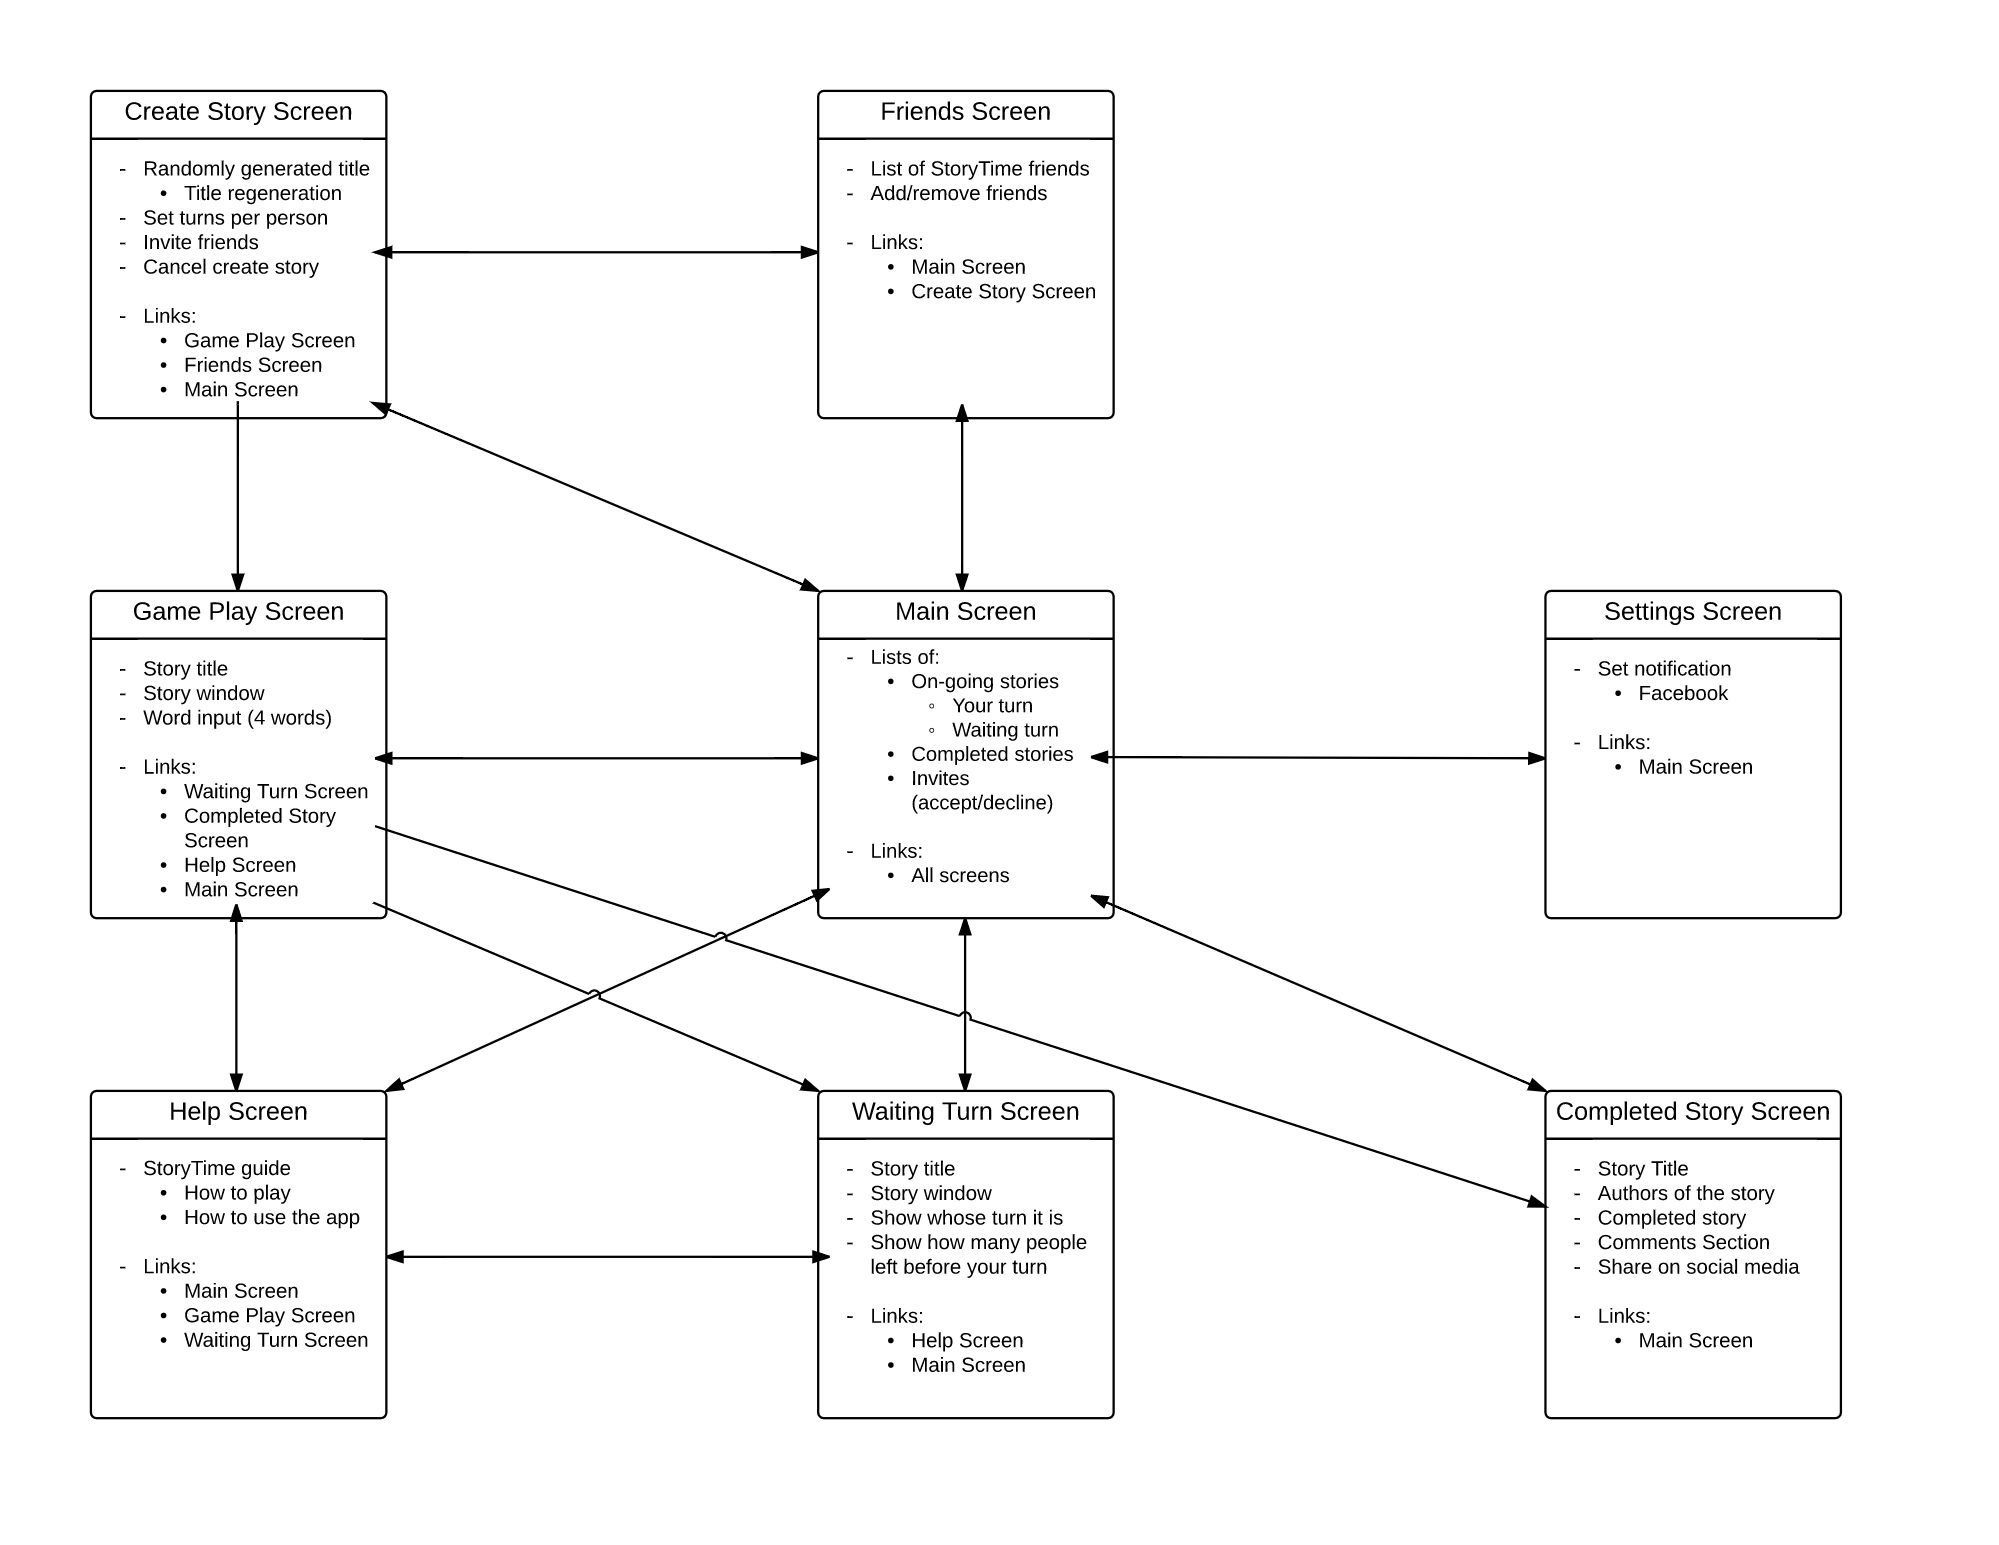
\includegraphics[width=\linewidth]{image00.png}
\caption{Conceptual Design for StoryTime With Friends}
\label{fig:conceptual}
\end{figure}




% ** ROLES AND RESPONSIBILITIES **

\onecolumn
\createappendix{Team Roles}\label{apx:roles}

\begin{table}[h!]
\centering
\begin{tabular}{>{\raggedright}p{4cm}|>{\raggedright}p{4cm}|>{\raggedright}p{6cm}}

\textbf{Team Member} &
\textbf{Project Role} &
\textbf{Responsibilities} \tabularnewline \hline \hline

Ali Dehghan &
Project Manager &
\begin{itemize}[leftmargin=.15in, nosep]
\item Making sure we move towards our motivation and we meet necessary research criteria
\item Joining user testing and interview sessions.
\item Writing methodology section of interim and final report.
\item Writing the MVC framework for implementation
\item Coding, testing and debugging the application.
\end{itemize} \tabularnewline \hline

Brandon Mabey &
Game Developer &
\begin{itemize}[leftmargin=.15in, nosep]
\item Implement and test minimum viable product.
\item Ensure consistency of user experience within StoryTime With Friends
\item Manage the Log-in system and ensure configuration of production server.
\item Research and write Background sections for interim and final reports.
\end{itemize} \tabularnewline \hline

Courtnay Low &
Business Analyst &
\begin{itemize}[leftmargin=.15in, nosep]
\item Wrote risks and team roles section for proposal.
\item Responsible for formatting and editing proposal.
\item Wrote distance work, milestones, risks and limitations for interim report.
\item Edited and rewrote various sections for interim and final report.
\end{itemize}\tabularnewline \hline

Sarah Warnock &
Application Designer &
\begin{itemize}[leftmargin=.15in, nosep]
\item Create the prototypes for user testing during design phase one.
\item Create conceptual design based off of user feedback from the prototype testing in design phase one.
\item Create interface for MVP using the conceptual design as a guide.
\item Research and write about related literature for interim and final report.
\item Write introduction for interim and final report.
\item Edit interim and final report.
\end{itemize} \tabularnewline \hline

Shaquille Davis &
Game Developer &
\begin{itemize}[leftmargin=.15in, nosep]
\item Implement color coding feature for the MVP.
\item Wrote limitations, questioniare analysis, and conclusion.
\item Coding some features of MVP.
\item Edit final report.
\end{itemize} \tabularnewline \hline

\end{tabular}
\caption{Roles and Responsibilities}
\label{tab:role}
\end{table}



\end{document}

%%% Local Variables:
%%% mode: latex
%%% TeX-master: t
%%% End:
